\documentclass[dvipdfmx]{jarticle}
\pagestyle{empty}
\usepackage{fancyvrb}
\usepackage{tikz}
\usetikzlibrary{shapes,calc,arrows.meta}
\begin{document}
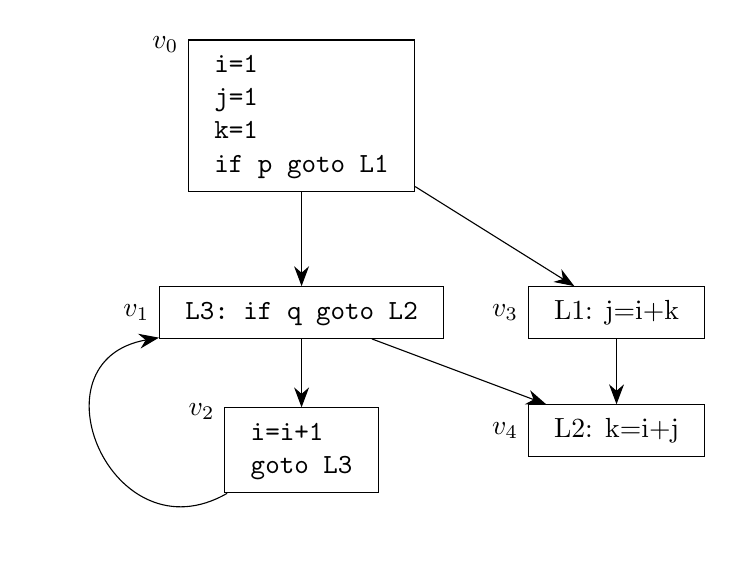
\begin{tikzpicture}
\node[draw,rectangle,label={155:{$v_0$}}] (v0) at (0,0) {\begin{tabular}{l}
\verb|i=1|\\
\verb|j=1|\\
\verb|k=1|\\
\verb|if p goto L1|
\end{tabular}};
\node[draw,rectangle,label={180:{$v_1$}}] (v1) at (0,-2.5) {\begin{tabular}{l}
\verb|L3: if q goto L2|
\end{tabular}};
\node[draw,rectangle,label={165:{$v_2$}}] (v2) at (0,-4.25) {\begin{tabular}{l}
\verb|i=i+1|\\
\verb|goto L3|
\end{tabular}};
\node[draw,rectangle,label={180:{$v_3$}}] (v3) at (4,-2.5) {\begin{tabular}{l}
L1: j=i+k
\end{tabular}};
\node[draw,rectangle,label={180:{$v_4$}}] (v4) at (4,-4) {\begin{tabular}{l}
L2: k=i+j
\end{tabular}};
\path[-{Stealth[scale=1.5]}] (v0) edge (v1) (v0) edge (v3);
\path[-{Stealth[scale=1.5]}] (v1) edge (v2) (v1) edge (v4);
\path[-{Stealth[scale=1.5]}] (v3) edge (v4);
\path[-{Stealth[scale=1.5]}] (v2) [out=210,in=190,looseness=2.0] edge (v1);
\end{tikzpicture}
\end{document}